\documentclass{article}
\usepackage{spconf,amsmath,amssymb,graphicx,booktabs,bm}
\usepackage{multirow}
\usepackage[hidelinks]{hyperref}
\usepackage{amsthm}
\newtheorem{theorem}{Theorem}

% ---- result macros (auto-generated from results/*.json; do not hand-edit numbers) ----
% target-specific certificate + calibration + baselines; NO fabrication/hallucination.
% AUTO-GENERATED by paper/emit_baseline_table.py -- do not hand-edit numbers.
\newcommand{\PhysMaxAngLo}{43}
\newcommand{\PhysMaxAngHi}{55}
\newcommand{\PhysMinAngLo}{2}
\newcommand{\PhysMinAngHi}{6}
\newcommand{\PhysMidAngLo}{10}
\newcommand{\PhysMidAngHi}{15}
\newcommand{\NTestFair}{800}
\newcommand{\FairSpanPriorQRS}{0.481}
\newcommand{\FairSpanDipQRS}{0.183}
\newcommand{\FairSpanRidgeQRS}{0.167}
\newcommand{\FairSpanUnetQRS}{0.164}
\newcommand{\FairLimbPriorQRS}{0.481}
\newcommand{\FairLimbRidgeQRS}{0.344}
\newcommand{\FairLimbUnetQRS}{0.238}
\newcommand{\FairUnetLimbSpanRatio}{1.46}
\newcommand{\RidgeUnetSpanCI}{$[-0.007,+0.000]$\,mV}
\newcommand{\SpanLimbUnetCI}{$[+0.070,+0.079]$\,mV}
\newcommand{\LadderQual}{a ladder in point estimates (the ridge$\to$U-Net step is within its paired CI)}
\newcommand{\EtaSTVone}{0.330}
\newcommand{\EtaNormVone}{0.740}
\newcommand{\AmbVone}{0.093}
\newcommand{\EtaSTVtwo}{0.712}
\newcommand{\EtaNormVtwo}{0.960}
\newcommand{\AmbVtwo}{0.200}
\newcommand{\EtaSTVthree}{0.553}
\newcommand{\EtaNormVthree}{0.955}
\newcommand{\AmbVthree}{0.155}
\newcommand{\EtaSTVfour}{0.268}
\newcommand{\EtaNormVfour}{0.534}
\newcommand{\AmbVfour}{0.075}
\newcommand{\EtaSTVfive}{0.084}
\newcommand{\EtaNormVfive}{0.170}
\newcommand{\AmbVfive}{0.024}
\newcommand{\EtaSTVsix}{0.027}
\newcommand{\EtaNormVsix}{0.057}
\newcommand{\AmbVsix}{0.007}
\newcommand{\SafetyN}{1498}
\newcommand{\SafetyFallbackPct}{14}
\newcommand{\FpDipolar}{5.3}
\newcommand{\FnDipolar}{45.7}
\newcommand{\TotDipolar}{51.1}
\newcommand{\ErrDipolar}{0.077}
\newcommand{\FpRidge}{1.7}
\newcommand{\FnRidge}{52.1}
\newcommand{\TotRidge}{53.7}
\newcommand{\ErrRidge}{0.076}
\newcommand{\FpOls}{1.7}
\newcommand{\FnOls}{51.8}
\newcommand{\TotOls}{53.5}
\newcommand{\ErrOls}{0.076}
\newcommand{\TotWrongLo}{51.1}
\newcommand{\TotWrongHi}{53.7}
\newcommand{\LWspearQRS}{1.00}
\newcommand{\LWspearQRSlo}{0.88}
\newcommand{\LWantlatQRS}{0.98}
\newcommand{\LWspearST}{0.89}
\newcommand{\LWspearSTlo}{-0.54}
\newcommand{\LWantlatST}{0.77}
\newcommand{\LWspearT}{0.94}
\newcommand{\LWspearTlo}{-0.66}
\newcommand{\LWantlatT}{0.72}
\newcommand{\LWSTTstable}{no}
\newcommand{\CalCov}{0.91}
\newcommand{\CalCovLo}{0.89}
\newcommand{\CalCovHi}{0.93}
\newcommand{\CalWidth}{0.150}
\newcommand{\WorstSubCov}{0.72}
\newcommand{\WorstSubName}{HYP}
\newcommand{\WorstSubN}{85}


\title{Target-Specific Recoverability Maps for Reduced-Lead ECG Reconstruction}
\name{Weiping Yan}
\address{University of Minnesota, Twin Cities}

\begin{document}
\maketitle

\begin{abstract}
Reconstructing missing electrocardiogram (ECG) leads from a reduced set is ill-posed, and
a scalar reconstruction error says nothing about \emph{which} named feature, on \emph{which}
lead, a clinician can trust. We give a \emph{target-specific recoverability map}: for a
waveform segment $s$ (P/QRS/ST/T), an observed lead set $S$, and a target lead $\ell$, two
closed-form numbers derived from one truncated SVD of the segment's empirical rank-3 spatial
(``dipolar'') sub-matrix---an \emph{identifiability} $\eta_{s,\ell}(S)$ (zero iff the
target's low-rank component is recoverable from $S$) and a \emph{conditioning}
$\kappa_{s,\ell}(S)$ (its noise/observed-residual gain). The per-lead criterion is the
classical estimability condition specialized to ECG, but made \emph{graded}: on PTB-XL the map
ranks target leads on a continuum---e.g.\ from limb leads, anterior precordial ST (V1--V4) is
not identifiable while lateral V5/V6 are near-identifiable---a call a physiological
precordial/limb split cannot make. It is stable to the truncation tolerance for well-posed
configurations and rank-sensitive (with reported sensitivity) for ill-posed ones. We attach
distribution-free calibrated intervals for the empirically predictable residual (conformalized
quantile regression, strict fold discipline, honestly stated within-group coverage), and give
a reconstructor-\emph{invariant} safety certificate: the total ST-threshold error floor is
near-invariant across reconstructors while the false-positive/false-negative split is a
design choice. The map turns ``trust the reconstruction'' into a per-feature, per-lead,
calibrated statement.
\end{abstract}

\begin{keywords}
electrocardiography, inverse problems, identifiability, conformal prediction,
trustworthy machine learning
\end{keywords}

\section{Introduction}
\label{sec:intro}
Wearable and reduced-lead ECG acquisition makes lead \emph{reconstruction} ubiquitous:
recover the standard 12 leads from one, three, or six observed leads
\cite{gradowski2025reveals,cardoso2024bayesian}. A low aggregate error certifies nothing
about \emph{which} morphological features are trustworthy: a cardiologist reads the P wave,
the QRS complex, the ST segment and the T wave, each on specific leads.

We ask a sharper, reconstructor-independent question: \emph{for a given observed lead set,
which target lead's dipolar morphology is even identifiable, and how well-conditioned is its
recovery?} Each waveform segment's instantaneous potential is approximately low rank across
leads; we estimate a per-segment rank-3 spatial basis $\bm M_s$ (top-3 singular vectors of
the population lead covariance). We stress that $\bm M_s$ is a \emph{population-estimated
(PCA)} object: on real PTB-XL it shares two directions with the classical
vectorcardiographic (inverse-Dower) dipole but its third direction differs materially, so we
call it an empirical rank-3 subspace rather than a physical dipole (Sec.~\ref{sec:exp}).

\noindent\textbf{Related work and contributions.} Classical work reconstructs missing leads
(regression / VCG synthesis \cite{edenbrandt1988dower,kors1990vcg,nelwan2004reduced}, deep
models \cite{gradowski2025reveals,cardoso2024bayesian}) or \emph{selects} optimal leads
\cite{joshi2009sensor}; whether a given target is even recoverable is the classical
estimability question \cite{scheffe1959anova}. None attaches a graded, per-target-lead
recoverability certificate with calibrated per-record error to a reconstruction. We do not
claim the underlying identity as new. Our contributions are: (1) a \emph{graded},
per-target-lead recoverability map---continuous $\eta_{s,\ell}(S)$/$\kappa_{s,\ell}(S)$ from a
single truncated SVD that \emph{rank} target leads (not a binary rank test), over an
\emph{empirically-estimated} $\bm M_s$ that differs $43$--$55^\circ$ from the textbook
inverse-Dower dipole, with a truncation-tolerance sensitivity analysis and record-bootstrap
CIs (Sec.~\ref{sec:cert}); (2) a calibration layer attaching distribution-free intervals
(a sound application of conformalized quantile regression + Mondrian \cite{romano2019cqr}, not
a new method) to the map per feature and lead, with strict fold discipline and honest
within-group (not per-diagnosis) coverage (Sec.~\ref{sec:calib}); (3) a
reconstructor-invariant safety certificate on PTB-XL---the total ST-threshold error floor is
near-invariant across reconstructors while the false-positive/false-negative split is a
design choice---showing anterior precordial ST is uncertifiable from limb leads
(Sec.~\ref{sec:exp}).

\section{The Recoverability Certificate}
\label{sec:cert}
% Exact per-target-lead identifiability (exact pseudo-inverse) vs the deployed rho-truncated
% numerical map. No residual-independence claim on real data; the strict lower bound is stated
% only for the synthetic model (Proposition 2).

\newtheorem{theoremc}{Proposition}
\newtheorem{propc}[theoremc]{Proposition}

% ---------------------------------------------------------------- setup
\noindent\textbf{Model.} Within segment $s$ write the population 12-lead vector as
$\bm L_s = \bm\mu_s + \bm M_s\bm d + \bm r_s$, where $\bm M_s\in\mathbb R^{12\times3}$
is the (population-estimated, PCA) dipolar basis, $\bm d$ the dipole coordinates, and
$\bm r_s$ the non-dipolar residual. Observing $S$ gives $\bm y_S=\bm{\mathrm{Sel}}_S\bm L_s
+\bm n$, with $\bm M_{s,S}=\bm{\mathrm{Sel}}_S\bm M_s$. Write the exact Moore--Penrose
pseudo-inverse $\bm M_{s,S}^{+}$ and the exact row-space projector
$\bm P_{\mathrm{obs}}=\bm M_{s,S}^{+}\bm M_{s,S}$. For numerical deployment we also use the
\emph{rank-$r$ truncation} at relative tolerance $\varrho$,
$\bm M_{s,S}^{(\varrho)}=\bm U_r\bm\Sigma_r\bm V_r^{\top}$ keeping singular triplets with
$\sigma_i>\varrho\,\sigma_{\max}$, with pseudo-inverse $\bm M_{s,S}^{(\varrho)+}$ and projector
$\bm P_{\mathrm{obs}}^{(\varrho)}=\bm V_r\bm V_r^{\top}$.

% ---------------------------------------------------------------- exact theorem
\begin{theoremc}[Exact per-target-lead dipolar identifiability and conditioning]
\label{thm:perlead}
For each target lead $\ell$ define
$\eta_{s,\ell}(S)=\big\|\bm e_\ell^{\top}\bm M_s(\bm I-\bm P_{\mathrm{obs}})\big\|_2$ and
$\kappa_{s,\ell}(S)=\big\|\bm e_\ell^{\top}\bm M_s\bm M_{s,S}^{+}\big\|_2$ from the \emph{exact}
$\bm M_{s,S}$.
\begin{enumerate}
\item[(i)] \emph{Identifiability.} $\eta_{s,\ell}(S)=0$ iff $\bm e_\ell^{\top}\bm M_s$ lies in
the exact row space of $\bm M_{s,S}$; then $\bm e_\ell^{\top}\bm M_s\bm d$ is a deterministic
function of $\bm M_{s,S}\bm d$---two dipoles with the same observation have the same lead-$\ell$
dipolar value, at any SNR. If $\eta_{s,\ell}(S)>0$ there is a $\bm\delta\in\ker\bm M_{s,S}$
(an unobserved dipole direction) with $\bm e_\ell^{\top}\bm M_s\bm\delta\neq0$; then $\bm d$ and
$\bm d+t\bm\delta$ produce identical observations for all $t$ while lead $\ell$'s dipolar value
changes, so it is not identifiable at any SNR.
\item[(ii)] \emph{Conditioning.} On the identifiable part, the lead-$\ell$ error from
observation noise and observed non-dipolar residual obeys
$\big|\bm e_\ell^{\top}\bm M_s\bm M_{s,S}^{+}(\bm{\mathrm{Sel}}_S\bm r_s+\bm n)\big|
\le \kappa_{s,\ell}(S)\,\big(\|\bm{\mathrm{Sel}}_S\bm r_s\|_2+\|\bm n\|_2\big).$
\end{enumerate}
The global $\kappa_s(S)=\|\bm M_s\bm M_{s,S}^{+}\|_2$ (spectral norm) upper-bounds every per-lead
$\kappa_{s,\ell}(S)$ (a row norm never exceeds the spectral norm; it is not their maximum).
\end{theoremc}

\noindent\emph{Exact vs.\ $\varrho$-identifiability (numerical deployment).} The deployed map
computes $\eta^{(\varrho)}_{s,\ell},\kappa^{(\varrho)}_{s,\ell}$ from the truncation
$\bm P_{\mathrm{obs}}^{(\varrho)}$, so a singular direction observed only through a value below
$\varrho\,\sigma_{\max}$ is treated as unobserved. Then $\eta^{(\varrho)}_{s,\ell}>0$ means lead
$\ell$ is \emph{not stably recoverable at resolution $\varrho$} (outside the retained numerical
row space); it does \emph{not} by itself imply the exact matrix has a null direction---a
tiny-but-nonzero singular value is exactly identifiable ($\eta=0$) yet $\varrho$-unidentifiable
($\eta^{(\varrho)}>0$), as we verify numerically (\texttt{tests/test\_exact\_vs\_rho.py}). We therefore call the
$\eta^{(\varrho)}$ heatmap the \emph{$\varrho$-identifiability} map; for well-separated
configurations the exact and $\varrho$ verdicts coincide, and near-rank-deficient $S$ are
reported with a $\varrho$-sweep and record-bootstrap CIs. \textbf{The limb-6 flagship is exact:}
the six limb leads are exact linear combinations of I and II (Einthoven/Goldberger), so
$\bm M_{s,S}$ has exact rank~2 and precordial ST is \emph{exactly} non-identifiable from limb
leads at any SNR, independent of $\varrho$.

\noindent\emph{Relation to classical estimability.} Part~(i) is the classical estimability
criterion (Gauss--Markov / \cite{scheffe1959anova}) for the linear functional
$\bm e_\ell^{\top}\bm M_s\bm d$; we claim no novelty for this identity. The contribution
(Sec.~\ref{sec:exp}) is its use as a graded, empirically-estimated recoverability map with
per-record calibrated error rates (Sec.~\ref{sec:calib}).

% ---------------------------------------------------------------- residual (honest)
\noindent\textbf{The non-dipolar residual (no independence claim on real data).}
Let $\bm m_s(\bm y_S)=\mathbb E[\bm r_s\mid\bm y_S]$ and
$\bm u_s=\bm r_s-\bm m_s(\bm y_S)$, so $\mathbb E[\bm u_s\mid\bm y_S]=\bm 0$. We do
\emph{not} assume $\bm u_s\perp\bm y_S$. Under squared loss the Bayes-optimal reconstruction
error of the (vector) residual is
\[
\inf_{\hat{\bm r}}\ \mathbb E\big\|\bm r_s-\hat{\bm r}(\bm y_S)\big\|_2^2
=\mathbb E\big[\operatorname{tr}\operatorname{Cov}(\bm r_s\mid\bm y_S)\big].
\]
Part of $\bm r_s$ (the \emph{empirically predictable residual}) is recovered by a
predictor trained on $\bm y_S$ and metered with distribution-free calibrated intervals;
the remainder is an \emph{achievability gap}, established by a held-out achievability
analysis for a stated predictor family---\emph{not} declared unrecoverable a priori.

\begin{propc}[Strict independence limit -- synthetic model only]
\label{prop:synth}
If the data are generated so that a component $\bm u$ is statistically independent of
$\bm y_S$ (an explicit synthetic construction), then $p(\bm u\mid\bm y_S)=p(\bm u)$, the
Bayes estimate of $\bm u$ under squared loss is its prior mean, and
$\mathbb E\|\widehat{\bm u}-\bm u\|_2^2\ge\operatorname{tr}\operatorname{Cov}(\bm u)$ for any
estimator. This strict limit is invoked \emph{only} for the synthetic model; on real ECG we
make no such independence claim.
\end{propc}


\section{Distribution-Free Calibration}
\label{sec:calib}
\textbf{Predictable-residual intervals.} For each pre-registered group $g=(S,s,\ell)$ we
train a quantile regressor of the target lead's off-dipole residual on the observed leads
(gradient-boosted pinball loss) and apply conformalized quantile regression
\cite{romano2019cqr} with a Mondrian (per-group) correction. Fold discipline is strict and
leakage-free: basis and quantile model on folds 1--7, conformal calibration on fold 9, a
single evaluation on fold 10. We report \emph{within-group marginal} coverage under
exchangeability (not per-example conditional coverage), interval width, and group sizes.

\textbf{Off-dipole flag.} We threshold the off-dipole energy at the one-sided $(1-\alpha)$
conformal quantile over faithful reconstructions; the false-flag rate is $\le\alpha$ for a
fresh reconstruction \emph{exchangeable with the calibration distribution}---not
distribution-free under an arbitrary shift.

\section{Experiments}
\label{sec:exp}
\textbf{Data.} PTB-XL \cite{wagner2020ptbxl} (21{,}799 twelve-lead records, 100/500\,Hz,
10-fold split) with P/QRS/ST/T delineation by NeuroKit2 \cite{makowski2021neurokit}.

\textbf{Reproducibility.} Code, fixed seeds, an exact environment lock, and a one-command
pipeline are released\footnote{Anonymized for review; released on acceptance.}; every number
in the tables is regenerated from result JSON (no hand-typed values). The neural baseline is a
24$\to$12-channel 1-D U-Net (base width 64, residual GroupNorm blocks, 60 epochs, Adam
$2{\times}10^{-4}$, MSE on masked leads under random lead masks); the residual predictor is a
gradient-boosted quantile regressor (pinball loss). The map is evaluated on records disjoint
from the folds used to estimate $\bm\mu_s,\bm M_s$.
\subsection{The recoverability map on PTB-XL}
We estimate $\bm M_s$ (rank 3; the cardiac dipole is 3-D \emph{a priori}, and the cumulative
explained variance confirms rank~3 captures the bulk---a rank-sensitivity sweep $r{=}2\dots5$ is
reported in \texttt{results/recoverability\_maps.json}) per segment on the training NORM records,
with RECORD-LEVEL bootstrap CIs (resample records, refit $\bm M_s$; $\varrho{=}10^{-2}$;
Fig.~\ref{fig:map}). We plot the \emph{normalized} identifiability
$\tilde\eta_{s,\ell}=\eta_{s,\ell}/\|\bm e_\ell^\top\bm M_s\|_2$---a dimensionless relative
unobserved geometric gain (a ratio of $L_2$ norms, not a variance fraction). A single observed
lead leaves every other lead unidentifiable; a dipole-spanning $\{$I,II,V2$\}$ or
$\{$I,II,V1,V3,V5$\}$ makes all targets \emph{exactly} identifiable ($\eta{=}0$).

\textbf{The robust flagship is exact.} The six limb leads are exact linear combinations of I and
II, so $\bm M_{s,S}$ for limb-6 has \emph{exact} rank 2: precordial ST is \emph{exactly}
non-identifiable from limb leads at any SNR, independent of $\varrho$ (Prop.~\ref{thm:perlead}).

\textbf{Graded ordering: stable for QRS, weighting-sensitive for ST/T.} A duplicated-limb
sensitivity analysis (\texttt{results/lead\_weighting.json}: refit on the 8 algebraically
independent leads, on the \emph{same} records) shows the V1--V6 $\tilde\eta$ ordering is
bootstrap-stable for QRS (Spearman $\LWspearQRS$, CI lower bound $\LWspearQRSlo$;
anterior-before-lateral in $\LWantlatQRS$ of resamples) but \emph{not} robust for the
low-amplitude ST/T segments (ST Spearman point $\LWspearST$ with a wide bootstrap CI;
anterior-before-lateral in only $\LWantlatST$ of resamples). We therefore report the ST/T
$\tilde\eta$/ambiguity magnitudes with this caveat and \emph{do not} claim a fine ST/T ordering;
the binary limb$\to$precordial verdict above is the robust ST statement. The estimated subspace
also depends on diagnosis (a NORM vs.\ MI principal-angle sensitivity is reported), so the map is
a \emph{NORM-trained reference}.

\begin{figure}[t]
  \centering
  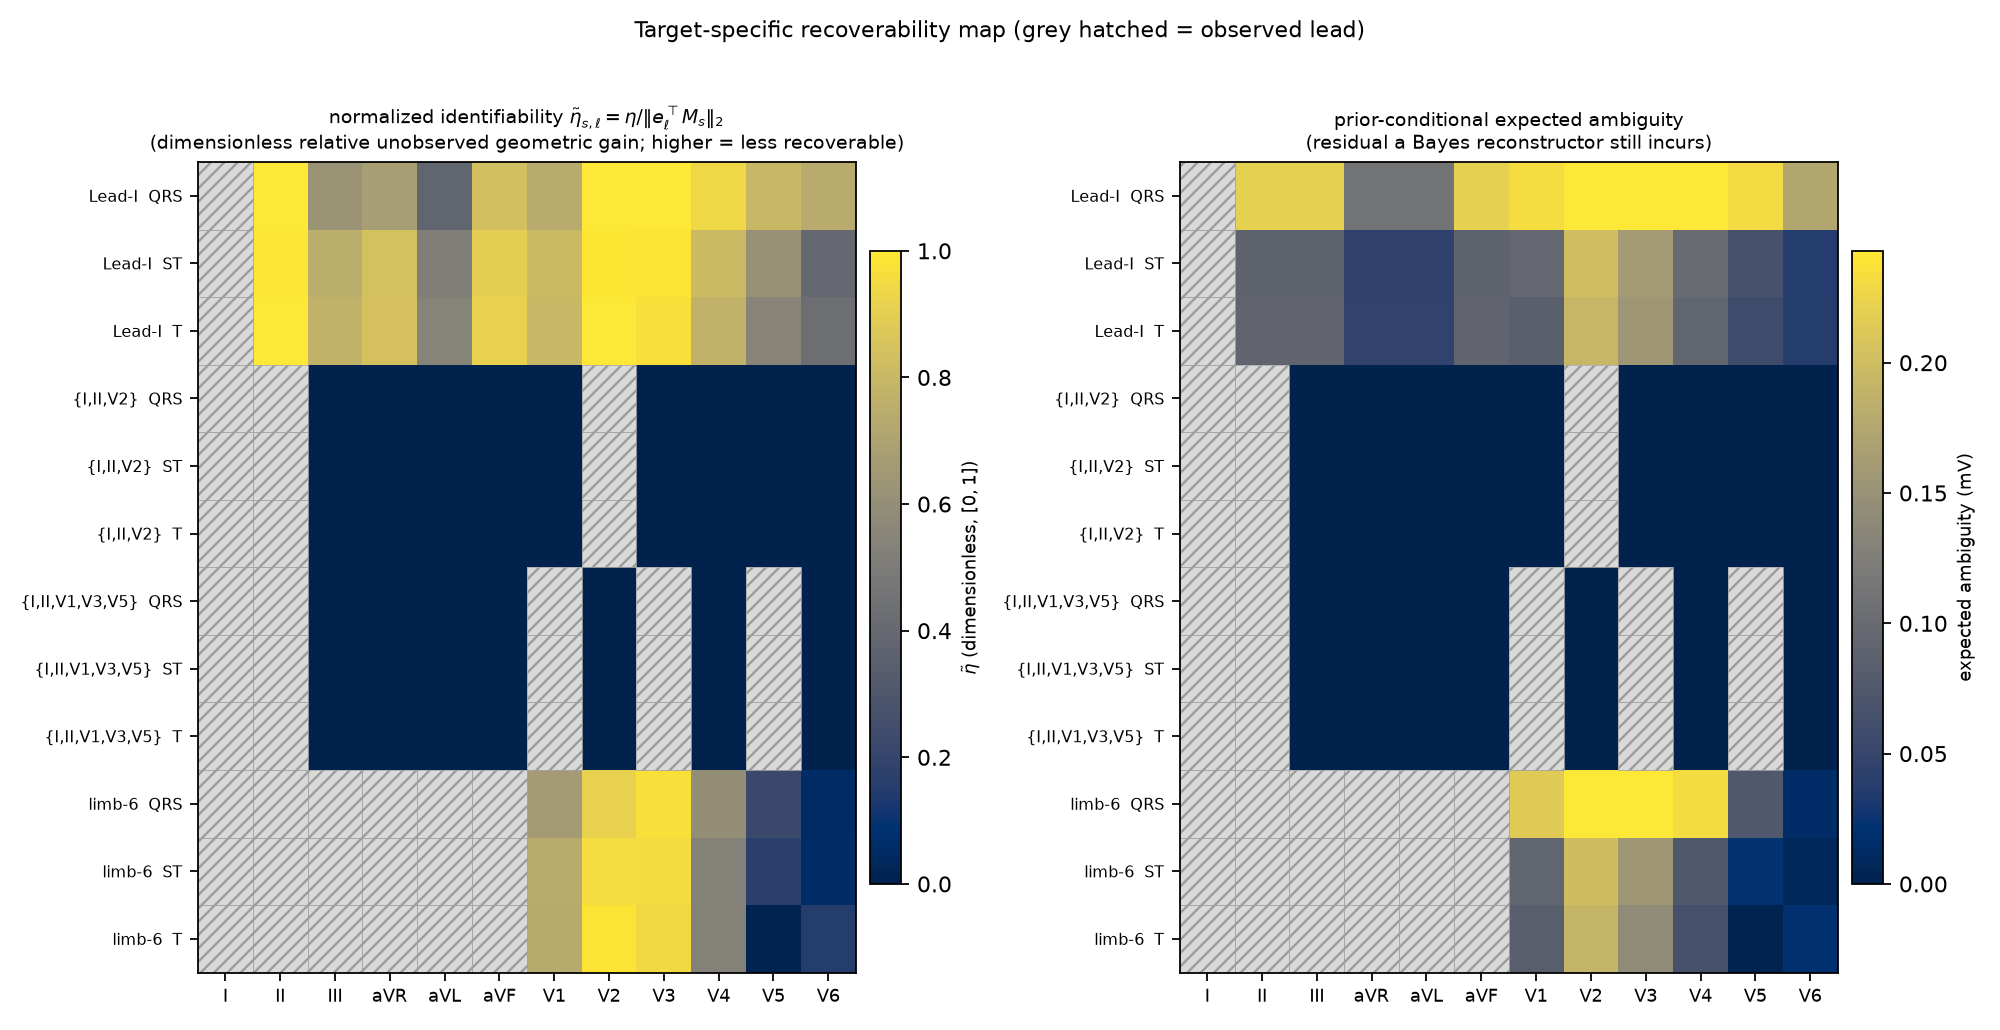
\includegraphics[width=\linewidth]{../results/recoverability_map.png}
  \caption{Recoverability map: normalized identifiability $\tilde\eta_{s,\ell}(S)$ (left,
  dimensionless) and prior-conditional expected ambiguity in mV (right), colorblind-safe
  \texttt{cividis}; grey hatched = observed. For limb-6 all precordial leads are unidentifiable
  ($\eta{>}0$); the fine ST/T ordering is weighting-sensitive (text).}
  \label{fig:map}
\end{figure}

\textbf{Downstream ST cost across reconstructors.} We reconstruct the full 10-second waveform
with three real continuous linear reconstructors (observed leads exact; ST at J$+$60\,ms vs.\ the
isoelectric PR-segment baseline [P offset\,--\,QRS onset], on fiducials from the observed Lead~II
shared between truth and reconstruction; median over beats; the PR-segment baseline fell back to
the pre-QRS window in $\approx\SafetyFallbackPct$\% of beats), and count ST-threshold events ($|$ST$|{\ge}0.1$\,mV; false positive =
crossing in reconstruction not truth, false negative = vice versa; Table~\ref{tab:safety}). On
$\SafetyN$ common records the \emph{total} wrong-event rate has point estimates ranging
$\TotWrongLo$--$\TotWrongHi\%$ across reconstructors and is \emph{dominated by false negatives}
(missed true crossings: limb$\to$precordial recovery smooths ST toward the population), with the
false-positive/false-negative split a reconstructor choice (paired record-bootstrap $\Delta$ on the
FP/FN split, and on the total, in \texttt{results/st\_safety.json}). We do not derive a minimax/Bayes
bound and make no equivalence claim: we report the range of total-error point estimates,
\emph{not} a certified lower bound, and ST-threshold events, not diagnoses. Because the PR-segment
baseline fell back to the pre-QRS window in $\approx\SafetyFallbackPct$\% of beats, the exact ST
magnitudes inherit that delineation limitation.

\begin{table}[t]
\centering\small
\caption{Limb-6 $\to$ precordial (all V1--V6) ST reconstruction, $\SafetyN$ common fold-10
records. FP/FN = false-positive/false-negative ST-threshold crossings (\%); total = FP+FN. FN
dominates (missed crossings); the split is a reconstructor choice. Auto-generated from
\texttt{results/st\_safety.json}.}
\label{tab:safety}
\begin{tabular}{lcccc}
\toprule
reconstructor & FP\,\% & FN\,\% & total\,\% & $|$ST$|$ err (mV) \\
\midrule
dipolar & \FpDipolar & \FnDipolar & \TotDipolar & \ErrDipolar \\
ridge   & \FpRidge   & \FnRidge   & \TotRidge   & \ErrRidge \\
OLS     & \FpOls     & \FnOls     & \TotOls     & \ErrOls \\
\bottomrule
\end{tabular}
\end{table}

\textbf{Truncation-tolerance sensitivity.} Well-posed configurations are $\varrho$-stable
($\{$I,II,V1,V3,V5$\}$ is rank~3 across $\varrho\!\in\!\{10^{-4},\dots,10^{-1}\}$); near-rank
-deficient sets are $\varrho$-sensitive and reported with the $\varrho$-sweep and bootstrap CIs.
A tiny-but-nonzero singular value is exactly identifiable yet $\varrho$-unidentifiable, which is
why we separate exact from $\varrho$-identifiability (Prop.~\ref{thm:perlead}).
\subsection{Calibrated intervals for the predictable residual}
The prediction target is the \emph{record-level segment-mean} off-dipole residual of the target
lead (one scalar per record: the mean over the segment's samples). We train a gradient-boosted
quantile regressor of it on the observed leads' segment means and apply Mondrian conformalized
quantile regression \cite{romano2019cqr} per $(S,s,\ell)$ group, with strict fold discipline:
basis and model on folds 1--7, the regressor's \texttt{max\_iter} selected by pinball loss on
fold 8, conformal calibration on fold 9, and a single evaluation on fold 10 (nominal
$1{-}\alpha{=}0.90$). This is a sound \emph{application} of established conformal machinery, not
a new predictor; the contribution is attaching it, per feature and lead, to the recoverability
map. Across the pre-registered $(S,s,\ell)$ groups, fold-10 within-group
coverage clusters near nominal ($0.87$--$0.94$; e.g.\ $\{$I,II,V1,V3,V5$\}$ QRS/V2
$\CalCov$, record-bootstrap CI $[\CalCovLo,\CalCovHi]$, mean width $\CalWidth$\,mV).

\textbf{What is and is not guaranteed.} Mondrian CQR gives \emph{within-$(S,s,\ell)$-group
marginal} coverage under exchangeability---\emph{not} coverage conditional on diagnosis, which
is not a conditioning variable. Diagnostic subgroups are therefore not guaranteed and the
smallest ones fall below nominal: the worst is the \WorstSubName{} subgroup at coverage
$\WorstSubCov$ ($n{=}\WorstSubN$), the expected finite-sample behaviour when conditioning on
a variable the calibration does not stratify on. We report worst-subgroup coverage rather than
hide it under the aggregate band, and we make no distribution-free claim beyond exchangeability
with the calibration fold.
\subsection{Baselines and what the map predicts}
Table~\ref{tab:base} reports reconstruction RMSE (mV) of the unobserved target leads under a
\emph{single, identical protocol} for all methods: per-timepoint waveform RMSE on the same
$\NTestFair$ held-out fold-10 records, same segment indices, record-bootstrap CIs. This is
the fair comparison---an earlier draft scored the classical baselines on segment-mean vectors
and the neural baseline on waveforms, which is not comparable. We include a \emph{strong
neural baseline}: an arbitrary-mask conditional 1-D U-Net trained with random lead masks (so
one model serves any configuration, no target-lead leakage), the masked-reconstruction
architecture the reduced-lead literature uses \cite{gradowski2025reveals}.

On a dipole-spanning set the methods form a monotone ladder---prior-mean $\to$ dipolar
(Tier~I) $\to$ per-segment ridge (Tier~I+II) $\to$ U-Net---confirming there is recoverable
non-dipolar content (the calibrated Tier~II layer), yet the strong neural model's margin over
a simple ridge is small (QRS $\FairSpanUnetQRS$ vs.\ $\FairSpanRidgeQRS$\,mV on
$\{$I,II,V1,V3,V5$\}$). The decisive result is on \textbf{limb-6}: \emph{every} reconstructor
degrades sharply, and the U-Net---despite its capacity---reaches only QRS $\FairLimbUnetQRS$,
$\FairUnetLimbSpanRatio\times$ its spanning-set error, still far above what it achieves when
the target is identifiable. No amount of model capacity crosses the identifiability ceiling
the map's $\eta{>}0$ warning marks out \emph{a priori}: limb$\to$precordial morphology is not
recoverable, so a low reconstruction error there would be spurious.

\begin{table}[t]
\centering\small
\caption{Reconstruction RMSE (mV) of target leads, QRS segment, under one identical
per-timepoint protocol ($\NTestFair$ test records). ``dipolar'' = Tier~I; ``ridge'' =
per-segment ridge (Tier~I+II); ``U-Net'' = strong arbitrary-mask neural baseline. Best in
bold. On limb-6 even the neural baseline cannot recover precordial morphology, as $\eta{>}0$
predicts. Numbers auto-generated from \texttt{results/fair\_baselines.json}.}
\label{tab:base}
% AUTO-GENERATED by paper/emit_baseline_table.py -- do not edit by hand.
\begin{tabular}{lcccc}
\toprule
config & prior-mean & dipolar & ridge & U-Net \\
\midrule
$\{$I,II,V2$\}$ & 0.471 & 0.234 & 0.220 & \textbf{0.181} \\
$\{$I,II,V1,V3,V5$\}$ & 0.484 & 0.186 & 0.168 & \textbf{0.164} \\
limb-6 & 0.484 & 0.362 & 0.346 & \textbf{0.239} \\
\bottomrule
\end{tabular}

\end{table}

\textbf{Empirical, not physical, dipole.} On real PTB-XL the estimated $\bm M_s$ shares two
directions with the classical inverse-Dower vectorcardiographic space (principal angles
$2$--$6^\circ$) but its third direction differs materially (max angle $43$--$55^\circ$,
bootstrap CIs excluding small angles). We therefore treat $\bm M_s$ as an \emph{empirical
rank-3 spatial subspace}, not a physical cardiac dipole; the earlier synthetic
``matches inverse-Dower'' check used inverse-Dower to generate the data and is not evidence
on real ECG. All certificate quantities are stated with respect to this estimated subspace.


\section{Conclusion}
Reduced-lead ECG reconstruction has a \emph{known low-rank structure per segment}. Exploiting
it gives a graded per-target-lead recoverability map---what is identifiable, how
well-conditioned, and (via calibration) what interval the predictable residual admits---before
and independent of any reconstructor. It tells a clinician which lead configuration can support
a decision, e.g.\ that anterior precordial ST cannot be read from limb leads while lateral
V5/V6 can, and reports the reconstructor-invariant error floor that any recovery must pay.

\bibliographystyle{IEEEbib}
\bibliography{refs}
\end{document}
